\documentclass[12pt,letterpaper]{article}
\usepackage{graphicx}
\usepackage{xfrac}
\usepackage{mcode}

\begin{document}

\title{Time-Frequency Analysis HW1}
\author{Beichen Su}

\maketitle

\begin{abstract}
A pratice emphiasize on denoise a nosiy moving signal of 3D by averaging white noise and gaussian filter.
\end{abstract}

\newpage
\section{Introduction and Overview}
Real life problem given:\\
You dog Fluffy swallowed a marble. The vet suspects that it has now worked its way into the intestines.
Using ultrasound, data is obtained concerning the spatial variations in a small area of the intestines where the
marble is suspected to be. Unfortunately, fluffy keeps moving and the internal fluid movement through the
intestines generates highly noisy data.\\
With a testdata contains 20 rows of data for 20 different measurements that were taken in time.
We tackle the problem by following steps:\\
1. Through averaging of the spectrum, determine the frequency signature (center frequency) generated by
the marble.\\
2. Filter the data around the center frequency determined above in order to denoise the data and determine
the path of the marble. (use plot3 to plot the path once you have it)\\
3. Find the position where should an intense acoustic wave be focused to breakup the marble at the 20th data measurement.\\
\newline 




\section{Theoretical Background}

Fast Fourier Transform: FFT, IFFT, FFTSHIFT, IFFTSHIFT\\
The transform can be calculated analytically so that we have the exact relations:\\

\begin{equation}
    \label{Fourier Transform}
    f(x) = \exp{(-\alpha x ^2)}  \rightarrow  \hat{f}(k) = \frac{1}{\sqrt(2\alpha)}exp(-\frac{k^2}{4\alpha})
\end{equation}

Given a function which has been discretized with $ 2^n $ points and represented by a vector x, the FFT is found with the command fft(x). Aside from transforming the function, the algorithm associated with the
FFT does three major things: it shifts the data so that $x \in [0, L] \rightarrow [−L, 0] 
$ and $x \in [−L, 0] \rightarrow [0, L] $, additionally it multiplies every other mode by −1, and
it assumes you are working on a $ 2pi $ periodic domain. (From course note)\\
Be simple, fourier tranform takes our signal function and tranforms it in the frequency domain, which has periodic boundary.







\section{Algorithm Implementation and Development}
To begin with we tackle the original data. For each row of data it was taken at different measurement in time, as we regrard it as a time snap shot. Each row of data contains 3D information so we reshape it into 3D matrix. Though the dog is moving that we cannot do anything with the spatial data for if we take the average the signal will disappear but we can take the average in the fourier domain so that the white noise will cancel out each other and we can find the max which represent the frequency signature of the marble, on which we put our filter.\\
Then we build a gaussian filter on the center frequency we find, loop again, reshape each row, take fast fourier transform of the signal, multiply it by the filter and transform it back to spatial domain. After these operation the signal in the spatial domain should not be noisy any more and by finding the max x,y,z spatial value we can locate the marble in space at each time step.
The 3D gaussian filter takes the form
\begin{equation}
    \label{Gaussian filter}
    Filter =  exp(-width*((Kx - Ka).^2+(Ky - Kb).^2+(Kz - Kc).^2));
\end{equation}
Where Kx,Ky,Kz are coordinate grid of frequency domain, and ka, kb, kc are the center frequency of marble we found by denoising.

\section{Computational Results}
1. Through averaging of the spectrum, determine the frequency signature (center frequency) generated by
the marble.\\
The frequency signature of marble takes 3 part in 3 dimension with 
\begin{equation}
	The revised central frequency is given as: 
Ka = 1.6755, Kb = -1.0472, Kc = 0.2094
\end{equation}
Corresponding to Kx, Ky, Kz in the code.\\
\newline
2. Filter the data around the center frequency determined above in order to denoise the data and determine
the path of the marble. \\
see Figure 1: Trajectory of marble\\
\begin{figure}
    \centering
    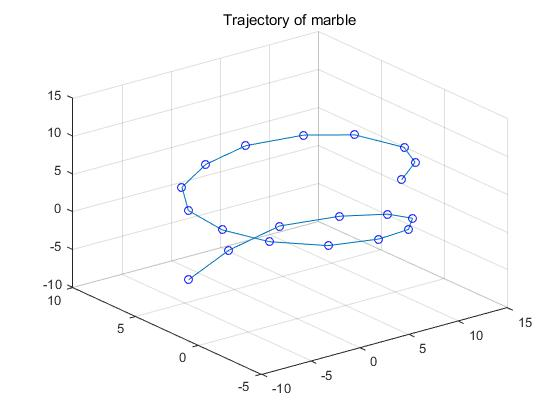
\includegraphics[width=3.0in]{r1}
    \caption{Trajectory of marble}
    
\end{figure}
3. Find the position where should an intense acoustic wave be focused to breakup the marble at the 20th data measurement.\\
At 20th data measurement, the marble is at $ (-5.6250 ,4.2188, -6.0938)$ in spatial coordinate.

\section{conclusion}
Knowing the fact that the frequency of a signal doesn't change whether the object change or not allow us to denoise a signal or determine if there is a signal or not. By applying the average and the filter method in fourier, the frequency domain, it's eazy to clear the noise and find our signal, and as a result, Fluffy is saved.


\appendix
\section{}
\subsection{linspace}
y = linspace(x1,x2,n) generates n points. The spacing between the points is (x2-x1)/(n-1).\\
In the code we have \\
$x2=linspace(-L,L,n+1);$\\
for FFT on a periodic boundary so the first point is the same as the last one. So we take n+1 mode and only pick the first n element.

\subsection{fft,fftshift,fftn}
fft,fft2,fftn transform the signal in 1D,2D and nD in to frequency domain with same dimension. When we do the tranformation, we must rescale the wavenumbers by $2*pi/L$ since the FFT assumes 2*pi periodic signals, where L is the spatial domain.

\subsection{meshgrid}
[X,Y,Z] = meshgrid(x,y,z) produces three-dimensional coordinate arrays. Make Matlab know your x, y ,z are perpendicular to each other.

\subsection{zeros, ones}
A = zeros(n,n,n) or ones(n,n,n) create a matrix with all zero and one entries with desired dimension

\subsection{reshape}
A = reshape(B,n,n) reshape a matrix with desired columns and rows

\subsection{max}
[m,I] = max(A);
A is a one dimensional matrix, m is the max number in the matrix and I is the index of m in A

\subsection{ind2sub}
The ind2sub command determines the equivalent subscript values corresponding to a single index into an array.
\section{}


\begin{lstlisting}
clear all; close all; clc;
load Testdata
L=15; % spatial domain
n=64; % Fourier modes
x2=linspace(-L,L,n+1); x=x2(1:n); y=x; z=x;
k=(2*pi/(2*L))*[0:(n/2-1) -n/2:-1]; 



[X,Y,Z]=meshgrid(x,y,z);
[Kx,Ky,Kz]=meshgrid(k,k,k);
Ufave = zeros(n,n,n);
% Reshape, fourier transform, add up in frequency domain 
% to cancel the white noise
for j=1:20
Un(:,:,:)=reshape(Undata(j,:),n,n,n);
Unf = fftn(Un);
Ufave(:,:,:) = Ufave + abs(Unf(:,:,:));
end

Ufave = Ufave/20;

% Find out the center frequency
Ufave = reshape(Ufave,n^3,1);
[m,I] = max(abs(Ufave));
[a,b,c] = ind2sub([n,n,n], I);

% Represent the center frequency in fourier domain
Ka = Kx(a,b,c);
Kb = Ky(a,b,c);
Kc = Kz(a,b,c);

% Build gaussian filter
width = 1;
Filter = exp(-width*((Kx - Ka).^2+(Ky - Kb).^2+(Kz - Kc).^2));
x = [];
y = [];
z = [];
% Bilter the noise out and save the position
% of marble at each snap shot
for j = 1:20
Un(:,:,:)=reshape(Undata(j,:),n,n,n);
Unf = fftn(Un);
Uf = Unf.*Filter;
U = ifftn(Uf);
U = reshape(U,n^3,1);
[m,I] = max(U);
[a,b,c] = ind2sub([n,n,n], I);
x(j) = X(a,b,c);
y(j) = Y(a,b,c);
z(j) = Z(a,b,c);

end
% Plot the path of marble
grid on;
plot3(x,y,z,'b--o ');
hold on;
grid on;

plot3(x,y,z)
title('Trajectory of marble')
PositionOfMarble = [x; y ;z];
% Last location
lastOne = PositionOfMarble(:,20);
\end{lstlisting}




































\end{document}